\subsection{Framework Overview}

Our DS-based ensemble framework transforms conventional ensemble learning into a principled evidence combination system. As illustrated in Figure~\ref{fig:framework}, the framework consists of three interconnected stages:

\begin{enumerate}
\item \textbf{Belief Assignment}: Converting softmax outputs from individual CNNs into DS mass functions
\item \textbf{Evidence Fusion}: Combining mass functions using Dempster's rule with conflict detection
\item \textbf{Decision Making}: Generating final predictions with comprehensive uncertainty metrics
\end{enumerate}

\begin{figure*}[t]
\centering
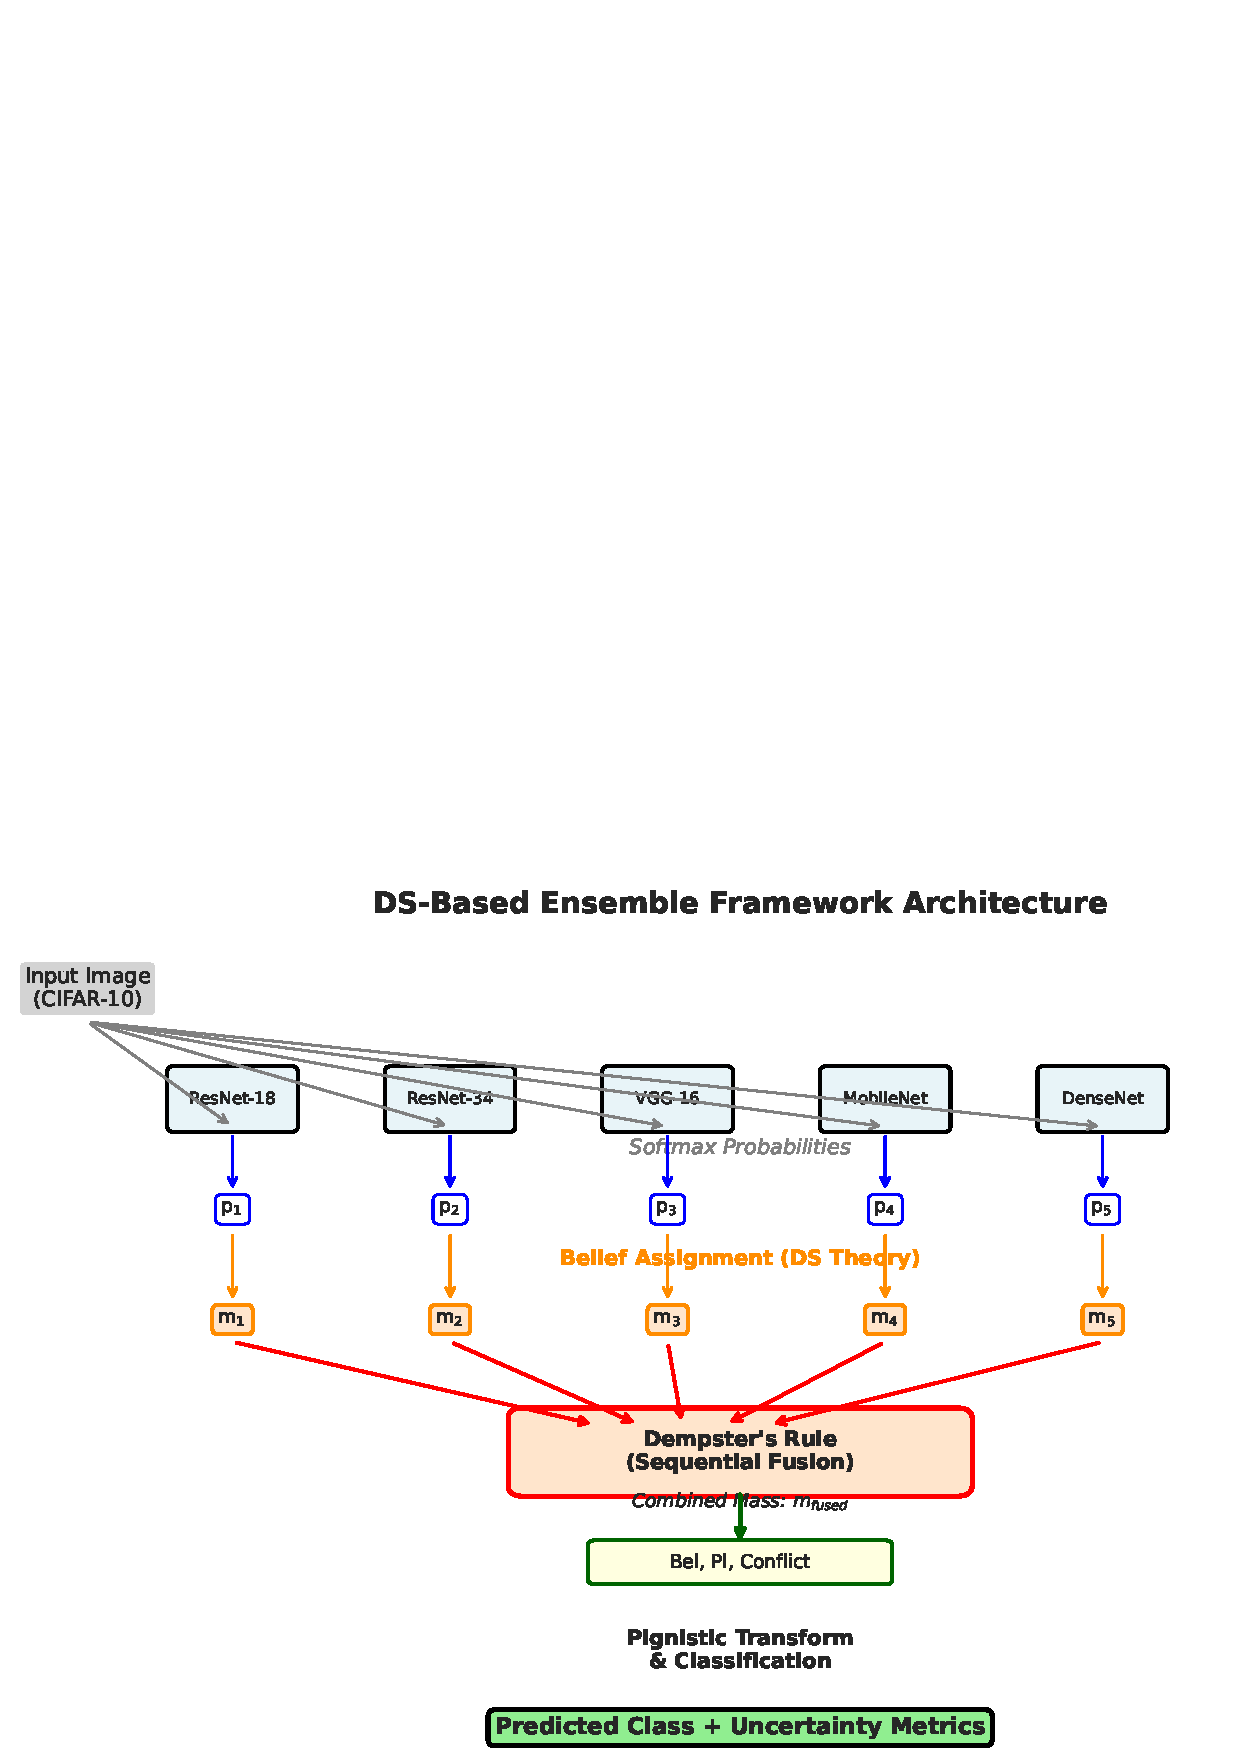
\includegraphics[width=0.95\textwidth]{../results/figures/framework_diagram.png}
\caption{Overview of our DS-based ensemble fusion framework. Individual CNN models generate softmax predictions, which are converted to belief mass functions. These masses are combined using Dempster's rule to produce a fused prediction with explicit uncertainty quantification including belief, plausibility, and conflict measures.}
\label{fig:framework}
\end{figure*}

Each component preserves deep learning's representational power while adding DS theory's uncertainty quantification capabilities. The framework is model-agnostic, working with any architecture producing probabilistic outputs.

\subsection{Post-Processing vs. Architectural Modification: Our Design Choice}
\label{sec:design_choice}

\textbf{Critical Clarification:} A fundamental question for any DS-based deep learning framework is whether it requires model retraining or can work as post-processing. We explicitly adopt a \textit{post-processing approach} that operates on standard softmax outputs from \textit{any pre-trained CNN models} without architectural modification or retraining.

\textbf{Comparison with Evidential Deep Learning (EDL):} Table~\ref{tab:our_vs_edl} contrasts our approach with EDL~\cite{sensoy2018evidential}, which represents an alternative paradigm for incorporating DS theory into deep learning.

\begin{table}[h]
\centering
\caption{Our Post-Processing Framework vs. Evidential Deep Learning}
\label{tab:our_vs_edl}
\small
\begin{tabular}{@{}lcc@{}}
\toprule
\textbf{Aspect} & \textbf{Our Method} & \textbf{EDL~\cite{sensoy2018evidential}} \\
\midrule
Input & Standard softmax & Modified output layer \\
Architecture & Unchanged & Dirichlet output \\
Training & Not required & New loss function \\
Pre-trained models & Compatible & Requires retraining \\
Black-box models & Applicable & Needs access \\
Ensemble needed & Yes (multi-model) & No (single model) \\
Computational cost & $<$1\% (inference) & Training + inference \\
Deployment time & Immediate & Weeks (retraining) \\
\bottomrule
\end{tabular}
\end{table}

\textbf{Advantages of Our Approach:}

\begin{enumerate}
\item \textbf{Immediate Deployment:} Works with existing pre-trained models (e.g., ImageNet models) without modification
\item \textbf{Black-Box Compatibility:} Only requires softmax outputs, enabling use with proprietary or third-party models
\item \textbf{Zero Training Cost:} Computational overhead applies only to inference (< 1\% vs. simple averaging)
\item \textbf{Ensemble Benefits:} Leverages model diversity across different architectures, training procedures, or initializations
\item \textbf{Practical Flexibility:} Can be applied/removed without system changes
\end{enumerate}

\textbf{Trade-offs:} EDL potentially captures uncertainty within a single model via Dirichlet parameterization, while our approach requires multiple models to quantify disagreement. However, ensemble diversity often provides richer uncertainty signals than single-model approaches~\cite{lakshminarayanan2017simple}.

\textbf{Computational Overhead Clarification:} The ``<1\% overhead'' cited in our abstract refers specifically to \textit{inference time} compared to averaging-based ensembles using the same models. Training costs are not increased because we use pre-trained models as-is. In contrast, EDL requires full model retraining with specialized loss functions, representing weeks of computational expense.

\subsection{From Softmax Probabilities to Basic Belief Assignments}

\textbf{The Conversion Challenge:} A critical question is how to transform CNN softmax outputs $\mathbf{p} = [p_1, p_2, \ldots, p_K]$ into DS basic belief assignments (BBAs). This conversion must preserve probabilistic information while enabling DS theory's uncertainty framework.

\textbf{Theoretical Justification:} In DS theory, a mass function $m: 2^\Theta \rightarrow [0,1]$ assigns belief to subsets of the frame of discernment $\Theta = \{c_1, \ldots, c_K\}$. For classification, we focus on singleton sets $\{c_i\}$ representing individual classes. The key insight is that softmax outputs already represent a form of evidence—model confidence in each class based on learned features. Our conversion interprets this confidence as belief mass.

Unlike Evidential Deep Learning~\cite{sensoy2018evidential}, which modifies network architecture to output Dirichlet distribution parameters, we work with standard softmax outputs. This design choice offers three advantages: (1) compatibility with pre-trained models, (2) no architecture modification required, and (3) applicability to black-box models.

\textbf{Conversion Strategies:} We propose three assignment strategies, each with different properties:

\textbf{1. Direct Assignment} (Distribution-Preserving):
\begin{equation}
m(\{c_i\}) = p_i, \quad \forall i \in \{1, \ldots, K\}
\label{eq:direct}
\end{equation}

This preserves the original probability distribution. For well-calibrated networks, direct assignment provides faithful evidence transfer. The remaining mass:
\begin{equation}
m(\Theta) = 1 - \sum_{i=1}^K m(\{c_i\})
\end{equation}
represents epistemic uncertainty—lack of evidence in the model.

\textbf{2. Temperature-Scaled Assignment} (Calibration-Adjusted):
\begin{equation}
m(\{c_i\}) = \frac{\exp(\log p_i / T)}{\sum_{j=1}^K \exp(\log p_j / T)}
\label{eq:temperature}
\end{equation}

Temperature scaling~\cite{guo2017calibration} adjusts confidence levels. For $T > 1$, the distribution smooths (reducing overconfidence); for $T < 1$, it sharpens. This addresses the common issue of overconfident neural networks, ensuring mass assignments reflect true prediction confidence.

\textbf{3. Calibrated Assignment} (Variance-Reducing):
\begin{equation}
m(\{c_i\}) = \frac{\sqrt{p_i}}{\sum_{j=1}^K \sqrt{p_j}}
\label{eq:calibrated}
\end{equation}

The square-root transformation reduces variance in probability estimates, useful for models with high confidence variation. This strategy provides a middle ground between direct and temperature-scaled approaches.

\textbf{Properties and Selection:} Our ablation studies (Section~\ref{sec:results}) show that for well-calibrated models (ResNet, DenseNet trained with standard procedures), direct assignment achieves optimal performance. Temperature scaling benefits overconfident models, while calibrated assignment helps when confidence varies significantly across predictions.

\subsection{Dempster's Rule of Combination}

Given mass functions $m_1$ and $m_2$ from independent sources (models), Dempster's rule combines them:
\begin{equation}
m_{1 \oplus 2}(A) = \frac{1}{1-\kappa} \sum_{B \cap C = A} m_1(B) m_2(C)
\label{eq:dempster}
\end{equation}

The conflict mass $\kappa$ measures disagreement:
\begin{equation}
\kappa = \sum_{B \cap C = \emptyset} m_1(B) m_2(C)
\label{eq:conflict}
\end{equation}

\textbf{Conflict Interpretation and Handling:} The conflict coefficient $\kappa \in [0,1]$ is not merely a normalization factor—it provides crucial information about model agreement. High conflict ($\kappa > 0.7$) indicates models fundamentally disagree, signaling:
\begin{itemize}
\item Ambiguous or difficult samples
\item Potential out-of-distribution inputs
\item Dataset boundary cases requiring careful handling
\end{itemize}

\textbf{Adaptive Conflict Management:} Based on conflict levels, we implement three handling strategies:

\begin{algorithm}[h]
\caption{Conflict-Aware Decision Policy}
\begin{algorithmic}[1]
\IF{$\kappa < 0.5$}
    \STATE \textbf{Low Conflict:} Use fused mass for prediction (models agree)
\ELSIF{$0.5 \leq \kappa < 0.7$}
    \STATE \textbf{Moderate Conflict:} Report wider uncertainty intervals
\ELSE
    \STATE \textbf{High Conflict:} Flag for human review or rejection
\ENDIF
\end{algorithmic}
\end{algorithm}

This adaptive policy enables deployment in safety-critical settings where uncertain predictions should be handled differently than confident ones.

For $N$ models, we apply Dempster's rule sequentially:
\begin{equation}
m_{combined} = m_1 \oplus m_2 \oplus \cdots \oplus m_N
\end{equation}

Recording conflict at each stage $\kappa_i$ provides a conflict profile showing where disagreements emerge.

\subsection{Uncertainty Quantification: Epistemic vs. Aleatoric}

DS theory naturally captures \textit{epistemic uncertainty} (model disagreement) distinct from \textit{aleatoric uncertainty} (inherent data noise). For hypothesis $A \subseteq \Theta$:

\textbf{Belief} (Lower probability bound):
\begin{equation}
Bel(A) = \sum_{B \subseteq A} m(B)
\end{equation}

\textbf{Plausibility} (Upper probability bound):
\begin{equation}
Pl(A) = \sum_{B \cap A \neq \emptyset} m(B)
\end{equation}

\textbf{Doubt} (Complement of plausibility):
\begin{equation}
Doubt(A) = 1 - Pl(A) = Bel(\neg A)
\end{equation}

The interval $[Bel(A), Pl(A)]$ captures epistemic uncertainty. Wide intervals indicate high model disagreement; narrow intervals suggest consensus. This differs from aleatoric uncertainty (data noise) which DS theory does not directly model—our focus is on uncertainty arising from ensemble disagreement.

\subsection{Decision Making and Uncertainty Reporting}

We use the pignistic transformation~\cite{smets1994transferable} to convert mass to probability:
\begin{equation}
P(c_i) = \sum_{A: c_i \in A} \frac{m(A)}{|A|}
\end{equation}

Final prediction:
\begin{equation}
\hat{y} = \arg\max_{c_i} P(c_i)
\end{equation}

For each prediction, we report:
\begin{itemize}
\item \textbf{Predicted class} $\hat{y}$ with pignistic probability $P(\hat{y})$
\item \textbf{Uncertainty interval} $[Bel(\{\hat{y}\}), Pl(\{\hat{y}\})]$
\item \textbf{Conflict measure} $\kappa$ averaged over fusion steps
\item \textbf{Interval width} $Pl(\{\hat{y}\}) - Bel(\{\hat{y}\})$ as uncertainty score
\end{itemize}

This comprehensive uncertainty profile enables nuanced decision policies unavailable to traditional ensembles.

\subsection{Reliability-Based Weighting}

For models with varying quality, we apply discount factors $\alpha_i \in [0,1]$ before fusion:
\begin{equation}
m_i'(A) = (1 - \alpha_i) m_i(A), \quad m_i'(\Theta) = m_i(\Theta) + \alpha_i (1 - m_i(\Theta))
\end{equation}

where $\alpha_i$ represents model $i$'s unreliability. We estimate:
\begin{equation}
\alpha_i = 1 - \text{Accuracy}_i^{val}
\end{equation}

Less reliable models contribute more mass to ignorance $\Theta$, preventing poor predictions from dominating the ensemble. This adaptive weighting naturally emerges from DS theory's discounting mechanism.
